\stepcounter{chapter} % This line will increment the chapter counter
\chapter*{Data Understanding and Preparation} % This line will create an unnumbered chapter
\addcontentsline{toc}{chapter}{\protect\numberline{\thechapter}Data Understanding and Preparation} % This line will add the chapter to your table of contents
\markboth{Data Understanding and Preparation}{} % This line will set the header
%\chapter{Data Understanding and Preparation}
\vspace{-10mm}
\section{Dataset}
The \textit{Spotify Tracks Dataset} used in this study contains information about audio tracks available in the Spotify catalog. These tracks span 20 different genres, such as chicago-house, black-metal and breakbeat. Each track is described by essential details (track's name, artist, album name, ...) and other features like its level of popularity within the Spotify catalog. The dataset also contains audio-derived features representing various aspects like danceability, energy, key, and loudness. The variables are specified in the table below:
\begin{footnotesize}
\begin{longtable}{|p{5cm}|p{6cm}|p{2cm}|}
\hline
\textbf{Name} & \textbf{Description} & \textbf{Type} \\
\hline
\endhead
\texttt{name} & Title of the track & \texttt{object}\\
\texttt{duration\_ms} & Track length in milliseconds & \texttt{int64} \\
\texttt{explicit} & Whether or not the track has explicit lyrics (True = yes; False = no/unknown) & \texttt{bool} \\
\texttt{popularity} & Popularity of a track (0 to 100) & \texttt{int64} \\
\texttt{artists} & Artist(s) who performed the track & \texttt{object} \\
\texttt{album\_name} & Album in which the track appears & \texttt{object} \\
\texttt{danceability} & How suitable a track is for dancing (0.0 to 1.0) & \texttt{float64} \\
\texttt{energy} & Perceptual measure of intensity and activity (0.0 to 1.0) & \texttt{float64} \\
\texttt{key} & Key of the track (standard Pitch Class notation) & \texttt{int64} \\
\texttt{loudness} & Overall loudness of the track in decibels (dB) & \texttt{float64} \\
\texttt{mode} & Modality (major or minor) of the track (major=1, minor=0) & \texttt{float64} \\
\texttt{speechiness} & Detects the presence of spoken words in the track & \texttt{float64} \\
\texttt{acousticness} & Confidence measure from 0.0 to 1.0 of whether the track is acoustic & \texttt{float64} \\
\texttt{instrumentalness} & Predicts whether a track contains no vocals & \texttt{float64} \\
\texttt{liveness} & Detects the presence of an audience in the recording & \texttt{float64} \\
\texttt{valence} & Musical positiveness conveyed by a track (0.0 to 1.0)& \texttt{float64} \\
\texttt{tempo} & Overall estimated tempo of a track in beats per minute (BPM) & \texttt{float64} \\
\texttt{features\_duration\_ms} & Duration of the track in milliseconds & \texttt{int64}\\
\texttt{time\_signature} & Estimated time signature & \texttt {float64}\\
\texttt{n\_beats} & Total number of time intervals of beats throughout the track & \texttt {float64}\\
\texttt{n\_bars} & Total number of time intervals of bars throughout the track & \texttt {float64}\\
\texttt {popularity\_confidence} & Confidence of the popularity of the song (0.0 to 1.0) & \texttt {float64}\\
\texttt{processing} & \textit{no information available}& \texttt{float64}\\
\hline
\end{longtable}
\end{footnotesize}
This report contains the summary of the analysis performed on the dataset in four stages: Data Understanding and Preparation, Clustering, Classification, Pattern Mining.

\section{Distribution of variables}
The dataset contains:
\begin{itemize}
    \item Continuous variables: duration\_ms, popularity, features\_duration\_ms, danceability, energy, loudness, speechiness, acousticness, instrumentalness, liveness, valence, tempo, n\_beats, n\_bars, popularity\_confidence.
    \item Discrete variables: key, processing and time\_signature.
    \item Categorical variables: mode and explicit (binary), name, artists, album\_name and genre (these will be label encoded in order to perform the analysis with all numerical columns).
\end{itemize}
\begin{figure}[H]
    \begin{minipage}{0.45\textwidth}
        \centering
        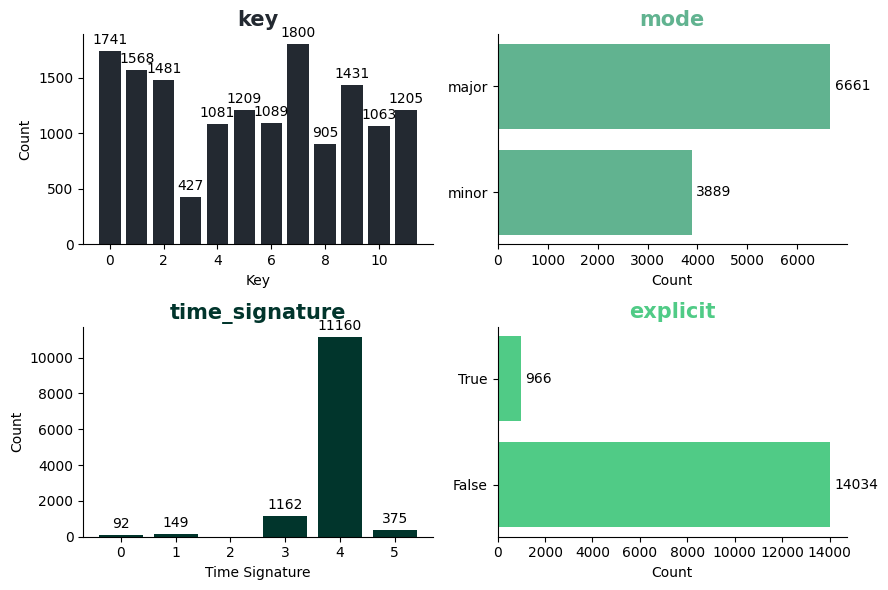
\includegraphics[scale=0.35]{img/categorical_bars.png}
        \caption{Distribution of discrete and binary variables.}
        \label{fig:enter-label}
    \end{minipage}
    \hfill
    \begin{minipage}{0.45\textwidth}
        \centering
        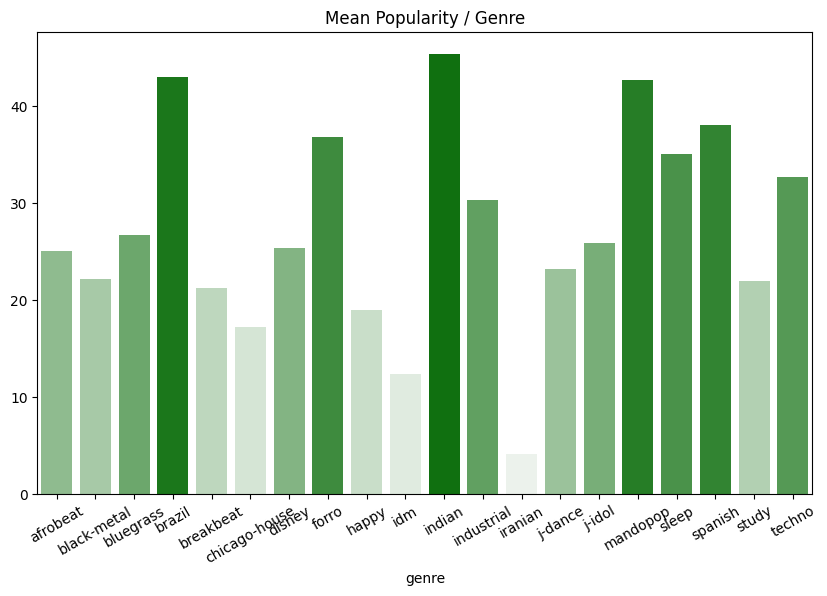
\includegraphics[scale=0.35]{img/popularity_genre.png}
        \caption{Mean popularity of tracks by genre.} 
        \label{fig:enter-label2}
    \end{minipage}
\end{figure}

Most of the tracks are in 4/4, and the keys C (0) and G (7) stand out, with a prevalence of major modes. Also noticeable is the sparse presence of songs with explicit content. By looking at the summary statistics of the continuous variables, we can calculate skewness and excess kurtosis. Excess kurtosis describes the shape of the tail of a distribution, while skewness measures the symmetry of the distribution. We can see that:
\begin{itemize}
\item \texttt{duration\_ms} has a high kurtosis ($161.5$) and positive skewness ($7.74$), indicating that most values are concentrated to the left of the mean with a long tail to the right;
\item \texttt{popularity}, \texttt{danceability}, \texttt{energy}, \texttt{acousticness}, \texttt{instrumentalness}, \texttt{val-\\*ence}, \texttt{tempo}, and \texttt{processing} have negative excess kurtosis, indicating that the distribution is flatter compared to a normal distribution;
\item \texttt{loudness}, \texttt{speechiness}, \texttt{liveness}, \texttt{n\_beats}, and \texttt{n\_bars} have positive excess kurtosis, indicating that the distribution has heavier tails and a sharper peak compared to a normal distribution;
\item There is no sufficient available data for \texttt{popularity\_confidence}.
\end{itemize}
\begin{comment}
\begin{figure}[!htb]
   \begin{minipage}{0.48\textwidth}
     \centering
     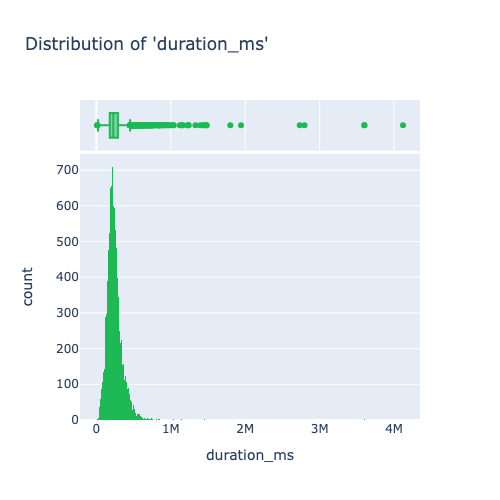
\includegraphics[width=\linewidth]{img/durationms_hist.png}
     \caption{Distribution of the feature 'duration\_ms'}\label{Fig:durationms_hist}
   \end{minipage}\hfill
   \begin{minipage}{0.48\textwidth}
     \centering
     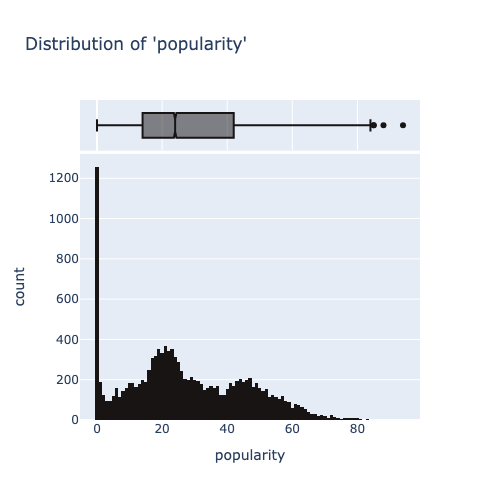
\includegraphics[width=\linewidth]{img/popularity_hist.png}
     \caption{Distribution of the feature 'popularity'}\label{Fig:popularity_hist}
   \end{minipage}
\end{figure}
\end{comment}

\section{Outliers detection}
\label{outliers_detection}
In order to check for possible outliers within the dataset, we can use some statistical tools, such as standard deviation and IQR (Interquartile Range), to measure the variability of data. The standard deviation method considers any data point that is a certain number of standard deviations away from the mean as an outlier; IQR is the range between the first and the third quartiles (namely $Q1$ and $Q3$): $\text{IQR} = Q3-Q1$. The data points which fall below $Q1-1.5*\text{IQR}$ or above $Q3+1.5*\text{IQR}$ may be candidate outliers.\\
We identified which features in the dataset have potential outliers according to both methods. We can view boxplots related to some of these features:
\begin{figure}[H]
    \centering
    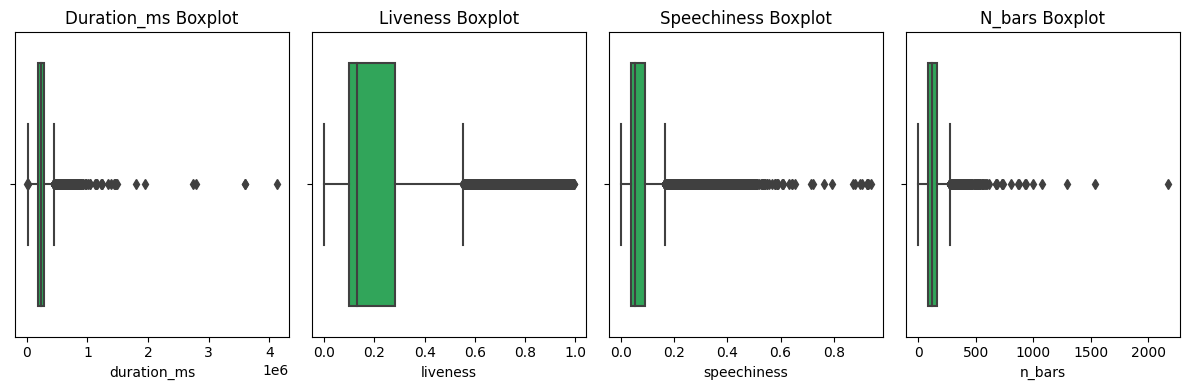
\includegraphics[scale=0.4]{img/boxplots.png}
    \caption{Some of the features with more presence of outliers according to the statistical methods used.}
    \label{fig:enter-label}
\end{figure}
The large presence of outliers for features such as \texttt{duration\_ms}, \texttt{liveness} and \texttt{speechiness} led us to check the details of the various candidate outliers: in fact, they actually refer to live recordings, DJ sets or compilations (like study background music). In this phase, we’ve decided not to remove any records, as doing so would result in a loss of approximately $44.59\%$ of the samples.
\newpage
\section{Handling missing values}
\begin{figure}[H]
    \centering
    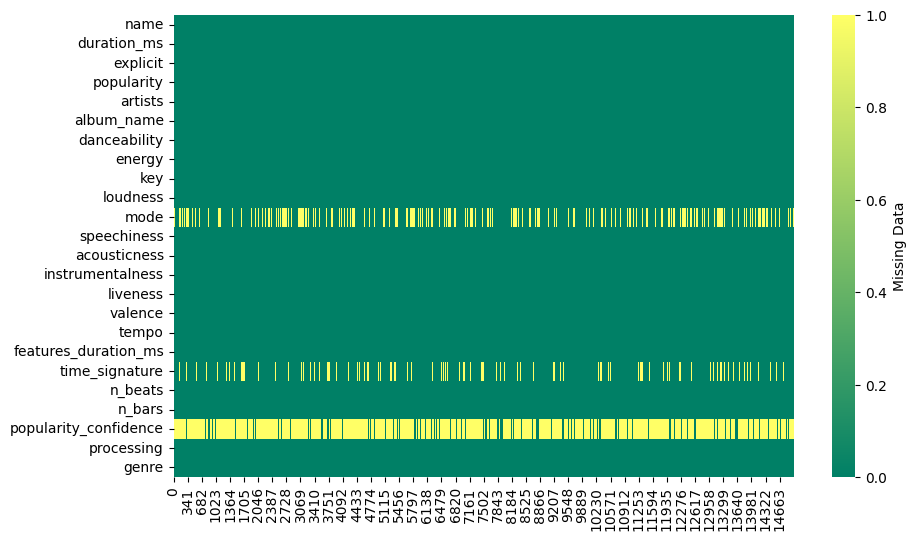
\includegraphics[scale=0.6]{img/missing_values.png}
    \caption{Heatmap of the data coded as boolean for "missing-ness" (1 is missing, 0 is not). Here we use the transposed boolean dataframe with \texttt{isna()} as input of the Seaborn’s \texttt{heatmap()} function.}
    \label{fig:missing-values}
\end{figure}
\begin{itemize}
\item \texttt{popularity\_confidence}: since 12783 values ($85.22\%$ of the total) turn out to be missing, we therefore decided to drop the column from the original dataset, because it may not contain any information about the data.
\item \texttt{mode}: the column contains binary values. Of these, $63.14\%$ are $1$ and $36.86\%$ are $0$. We decided to replace the null values by randomly inserting $0$ or $1$ while maintaining the percentage of the two classes. Although it might be formally wrong to assign 'minor' or 'major' even to track types such as live recordings or compilations, we noticed that among the nonmissing records it had already been done, so we simply chose to keep the percentage of classes. In this way we prevented the deletion of records that could be used in the next analysis and at the same time maintained the distribution of classes without altering the dataset.
\item \texttt{time\_signature}: we checked the Spotify Web API documentation in order to get more specific information about the variables. In the "Tracks" section, time\_signature is described as an estimated time signature ranging from 3 to 7, indicating time signatures from "3/4" to "7/4" . Time signature (or meter) is a notation convention for specifying the number of beats in each measure (or measure). So we may decide to reject the variable, as it can be calculated from two other variables in the dataset (n\_beats and n\_bars). In order to verify this choice, we tested the calculation on a copy of the dataset, filtered with only non null values. The accuracy is calculated as the percentage of recalculated values corrected (i.e., with the value equal to the true value of time\_signature). The result is: \mintinline{python}|Accuracy Rate: 95.90|\%. We can therefore consider the formula reliable and drop the column as the feature can be derived.
\end{itemize}

\section{Dependencies and correlations}
\begin{figure}[H]
    \centering
    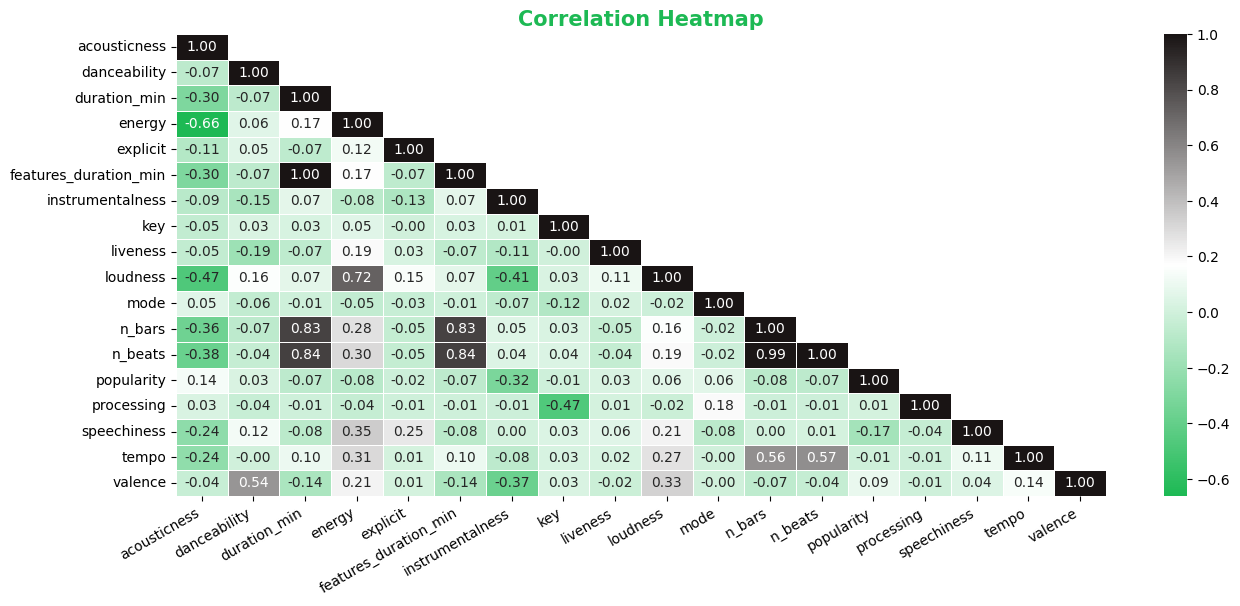
\includegraphics[scale=0.45]{img/corr_heatmap.png}
    \caption{Spearman's correlation heatmap of features.}
    \label{fig:enter-label}
\end{figure}
After dropping duration\_ms and features\_duration\_ms because durations in minutes were introduced, we can see that the correlation matrix confirms that longer songs typically have more beats and bars. Energetic songs tend to be louder, while acoustic songs have lower energy. Instrumental tracks generally have lower energy and loudness. Valence is positively related to danceability and tempo, suggesting happier songs are more danceable and faster-paced. Faster-tempo songs are also more danceable. We can also drop the "features\_duration\_min" column because it has virtually maximum positive correlation with "duration\_min".\\
\\
Once we had filtered the dataset by selecting and standardizing (using the StandardScaler from \texttt{sklearn.preprocessing}) only continuous variables, we decided to implement a PCA (from \texttt{sklearn.decomposition}) to look for additional relationships between variables and identify the linear combinations of original variables that explain most of the variance in the data. After visualizing the scree plot, considering the elbow rule, we can rerun the PCA with 3 components and interpret the results. The results of the PCA, and the loadings of the original variables on the first three principal components are organized into new dataframes. \\
This procedure leads to the following results:
\begin{figure}[H]
    \begin{minipage}{0.5\textwidth}
        \centering
        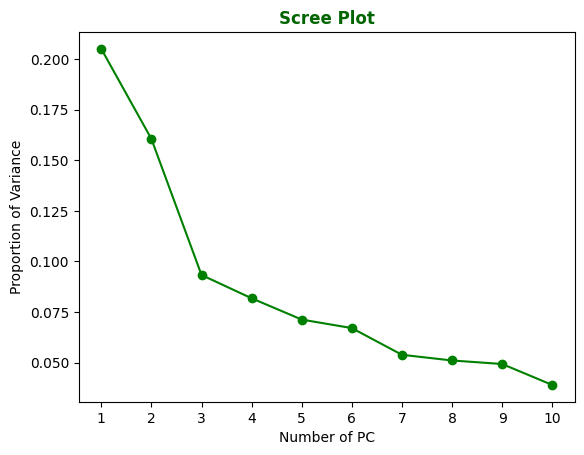
\includegraphics[scale=0.4]{img/scree_plot.png}
        \caption{The scree plot shows how much each principal component contributes to the total variance of the data.}
    \end{minipage}
    \hfill
    \begin{minipage}{0.5\textwidth}
        \begin{table}[H]
            \tiny
                \centering
            \begin{tabular}{|l|l|l|l|}
                \hline
                \textbf{Feature} & \textbf{PC1} & \textbf{PC2} & \textbf{PC3} \\
                \hline
acousticness & -0.36 & 0.14 & 0.03 \\
danceability & 0.15 & \textbf{-0.33} & 0.00 \\
duration\_min & 0.31 & \textbf{0.39} & 0.02 \\
energy & \textbf{0.39} & -0.23 & -0.02 \\
explicit & 0.06 & -0.14 & -0.04 \\
instrumentalness & -0.14 & 0.31 & -0.15 \\
key & 0.05 & -0.03 & \textbf{-0.62} \\
liveness & 0.03 & -0.03 & 0.04 \\
loudness & 0.36 & -0.33 & 0.04 \\
mode & -0.04 & 0.02 & 0.36 \\
n\_bars & \textbf{0.40} & \textbf{0.38} & 0.04 \\
n\_beats & \textbf{0.41} & 0.36 & 0.04 \\
popularity & -0.04 & -0.11 & 0.13 \\
processing & -0.03 & 0.02 & \textbf{0.65} \\
speechiness & 0.06 & -0.15 & -0.08 \\
tempo & 0.31 & -0.00& 0.05 \\
valence& 0.15& \textbf{-0.37}& 0.06\\
                \hline
            \end{tabular}
            \caption{Principal Component Loadings}
        \end{table}
    \end{minipage}
\end{figure}
\noindent PC1 is influenced by n\_beats, n\_bars, and energy, so it might be viewed as a measure of the rhythm intensity of the track. PC2 is positively influenced by duration\_min and n\_bars, and negatively influenced by valence and danceability: it might be seen as contrasting measure of song duration and rhythm structure with the mood and danceability of the music. PC3 is influenced by processing and negatively influenced by key, it might be viewed as a measure of the key’s impact on the processing of the music. This is an interpretation of the results with the understanding that PCA is a "black box": since we do not know the procedure behind the algorithm's choice of PCs, we are giving a hypothesis that can later be confirmed or discarded during. Before continuing, we can further select the variables in the dataset: as we dropped time\_signature, by the same reasoning we can drop n\_beats, because it can be derived from the product $\texttt{duration\_min}*\texttt{tempo}$ (which is in fact expressed in beats per minute, BPM). Entering the second phase of the analysis, we decided to normalize all variables using Z-Score normalization (\texttt{StandardScaler} class from the \texttt{sklearn.preprocessing} module), since is less sensitive than Min-Max to the presence of outliers. This is the description of the dataset at the end of the data understanding phase:\\
\begin{center}
\begin{tiny}
\begin{tabular}{|l|l|l|l|l|l|l|l|l|l|}
\hline
\textbf{index} & \textbf{count} & \textbf{mean} & \textbf{std} & \textbf{min} & \textbf{25\%} & \textbf{50\%} & \textbf{75\%} & \textbf{max} \\
\hline
name & 15000 & 7499.5 & 4330.271 & 0 & 3749.75 & 7499.5 & 11249.25 & 14999 \\
explicit & 15000 & 0.064 & 0.245 & 0 & 0 & 0 & 0 & 1 \\
popularity & 15000 & 0 & 1 & -1.475 & -0.722 & -0.184 & 0.784 & 3.582 \\
artists & 15000 & 1987.648 & 1755.411 & 0 & 486 & 1437 & 3178 & 6256 \\
album\_name & 15000 & 4084.496 & 2832.827 & 0 & 1569.75 & 3673 & 6399 & 9819 \\
danceability & 15000 & 0 & 1 & -2.837 & -0.567 & 0.149 & 0.741 & 2.208 \\
energy & 15000 & 0 & 1 & -2.482 & -0.667 & 0.2 & 0.862 & 1.3 \\
key & 15000 & 0 & 1 & -1.475 & -0.917 & -0.08 & 0.757 & 1.593 \\
loudness & 15000 & 0 & 1 & -6.766 & -0.29 & 0.265 & 0.632 & 2.007 \\
mode & 15000 & 0.628 & 0.483 & 0 & 0 & 1 & 1 & 1 \\
speechiness & 15000 & 0 & 1 & -0.966 & -0.536 & -0.378 & 0.056 & 9.863 \\
acousticness & 15000 & 0 & 1 & -0.922 & -0.893 & -0.452 & 0.817 & 2.1 \\
instrumentalness & 15000 & 0 & 1 & -0.749 & -0.749 & -0.741 & 1.194 & 1.863 \\
liveness & 15000 & 0 & 1 & -1.11 & -0.609 & -0.439 & 0.324 & 3.98 \\
valence & 15000 & 0 & 1 & -1.576 & -0.869 & -0.075 & 0.819 & 2.013 \\
tempo & 15000 & 0 & 1 & -3.856 & -0.726 & 0.034 & 0.591 & 3.051 \\
n\_bars & 15000 & 0 & 1 & -1.709 & -0.604 & -0.152 & 0.407 & 27.181 \\
processing & 15000 & 0 & 1 & -1.197 & -0.848 & -0.38 & 0.948 & 1.54 \\
genre & 15000 & 0 & 1 & -1.648 & -0.824 & 0 & 0.824 & 1.648 \\
duration\_min & 15000 & 0 & 1 & -1.861 & -0.522 & -0.148 & 0.329 & 30.264 \\
\hline
\end{tabular}
\end{tiny}
\end{center}


